% ============================================================
%  TERM PROJECT – PROPOSAL (template)
%  Databases · THGA Bochum
%
%  How to use:
%    1. Copy this folder into your own repository.
%    2. Replace every  <<< ... >>>  placeholder with your content.
%    3. Build with  `make`  (see the Makefile / README).
%    4. Send the resulting PDF to the lecturer and wait for approval.
% ============================================================
\documentclass[11pt,a4paper]{article}

\usepackage{thga-db}
\usepackage{caption}   % enables \captionof inside minipages

% ----- Fill in your metadata -------------------------------
\renewcommand{\thgaKurs}{Databases}
\renewcommand{\thgaDatum}{Summer Term 2026}
\newcommand{\authorName}{<<< Your name >>>}
\newcommand{\projectTitle}{<<< Working title of your application >>>}

\begin{document}
\thispagestyle{empty}
\thgaTitel{Term Project – Proposal}{\projectTitle}

\begin{infobox}
\textbf{Author:} \authorName \\
\textbf{Module:} Introduction to Database Management Systems · THGA Bochum \\
\textbf{Submitted to:} Stephan Bökelmann · \href{mailto:sboekelmann@ep1.rub.de}{sboekelmann@ep1.rub.de} \\
\textbf{Target size:} about 6 pages
\end{infobox}

\begin{infobox}
\textbf{Every figure must be explained in the running text.} A figure never
stands on its own: refer to it by number and say what it shows -- e.g.
``Figure~\ref{fig:er} shows the ER model of \dots''.

Every figure below is \texttt{example-figure.jpg}, a dummy image shipped with
this template. Photograph or scan your own sketch, drop the file next to
\texttt{proposal.tex}, and point \texttt{\textbackslash includegraphics} at it:
\begin{quote}
\texttt{\textbackslash includegraphics[width=0.85\textbackslash linewidth]\{er-sketch.jpg\}}
\end{quote}
The \texttt{width} option scales the image to a fraction of the text width; the
file extension may be omitted. Keep the \texttt{\textbackslash caption} and the
\texttt{\textbackslash label} as they are.
\end{infobox}

% ============================================================
\section{Application domain and motivation}
% ============================================================

<<< Which application do you build and which problem does it solve? Who uses
it, and for what? Add one or two concrete usage scenarios. >>>

% ============================================================
\section{Data model -- ER sketch}
% ============================================================

\begin{figure}[ht]
  \centering
  % Swap example-figure.jpg for your own file, e.g. er-sketch.jpg
  % (a photographed hand drawing is fine).
  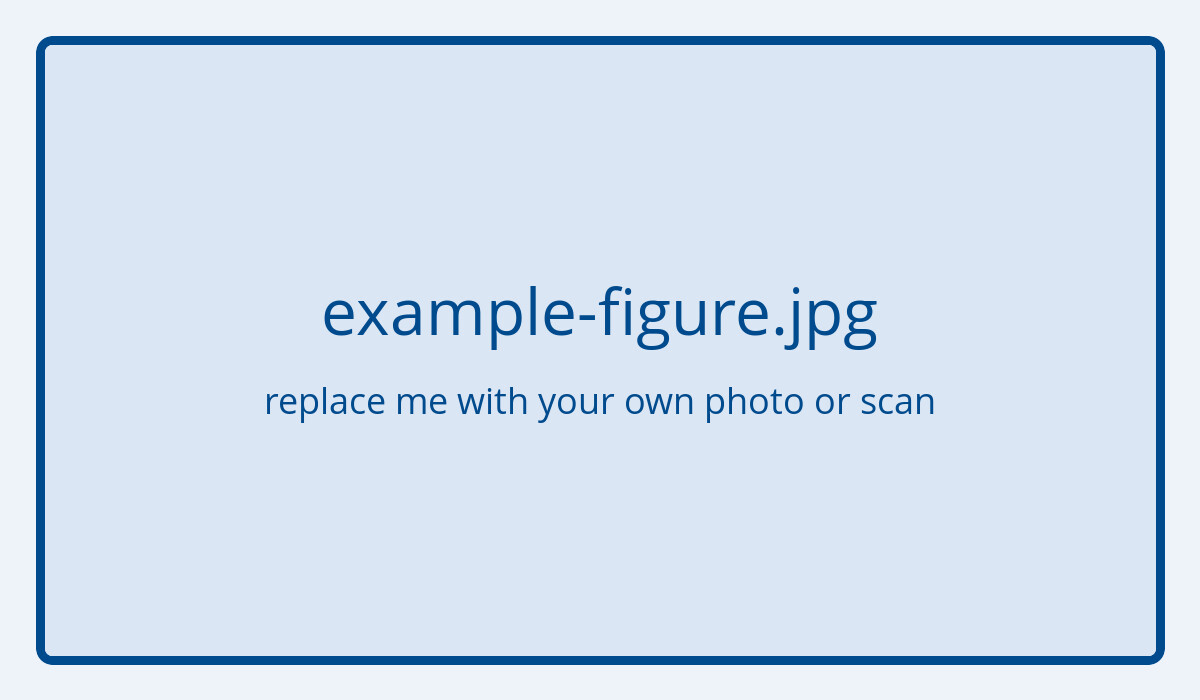
\includegraphics[width=0.85\linewidth]{example-figure.jpg}
  \caption{ER sketch of the <<< domain >>> data model: entity types, key
  attributes, relationships and cardinalities (at least one N:M).}
  \label{fig:er}
\end{figure}

Figure~\ref{fig:er} shows <<< explain your ER model here: name the central
entity types, the key attributes and the relationships, and point out the N:M
relationship and its cardinalities. >>>

% ============================================================
\section{From model to schema}
% ============================================================

<<< Derive the relational schema. For each table give the columns, the primary
key (underlined) and the foreign keys. >>>

\begin{itemize}
  \item \texttt{<<<table>>>}(\underline{id}, <<<column>>>, \dots)
  \item \texttt{<<<table>>>}(\underline{id}, \emph{<<<foreign\_key>>>}, \dots)
\end{itemize}

\textbf{Normalisation.} <<< One or two sentences: why is the schema free of
redundancy (at least 3NF)? >>>

% ============================================================
\section{API design}
% ============================================================

<<< List the planned FastAPI endpoints. Mark where a JOIN / an aggregation
sits, and which endpoints require the X-API-Key. >>>

\renewcommand{\arraystretch}{1.2}
\begin{tabularx}{\linewidth}{@{}p{2cm}p{4cm}X@{}}
\toprule
\textbf{Method} & \textbf{Path} & \textbf{Purpose} \\
\midrule
\texttt{GET}  & \texttt{/<<<…>>>} & <<< reads … (JOIN / aggregation) >>> \\
\texttt{POST} & \texttt{/<<<…>>>} & <<< creates … (requires X-API-Key) >>> \\
\bottomrule
\end{tabularx}

% ============================================================
\section{Frontend prototype (hand sketches)}
% ============================================================

<<< Describe what the frontend looks like and which endpoints it operates, and
document a prototypical frontend with hand-drawn sketches -- one per screen/form.
Python/tkinter is recommended; if you use something else, say what and why. The
frontend is delivered as a .deb installer and asks for the API URL and X-API-Key
in a connection dialog at startup. >>>

% Each \includegraphics below still points at the dummy example-figure.jpg.
% Swap in your own file per screen, e.g. {fe-connect.jpg}, and keep the \captionof.
\begin{figure}[ht]
\centering
\begin{minipage}[t]{0.47\linewidth}\centering
  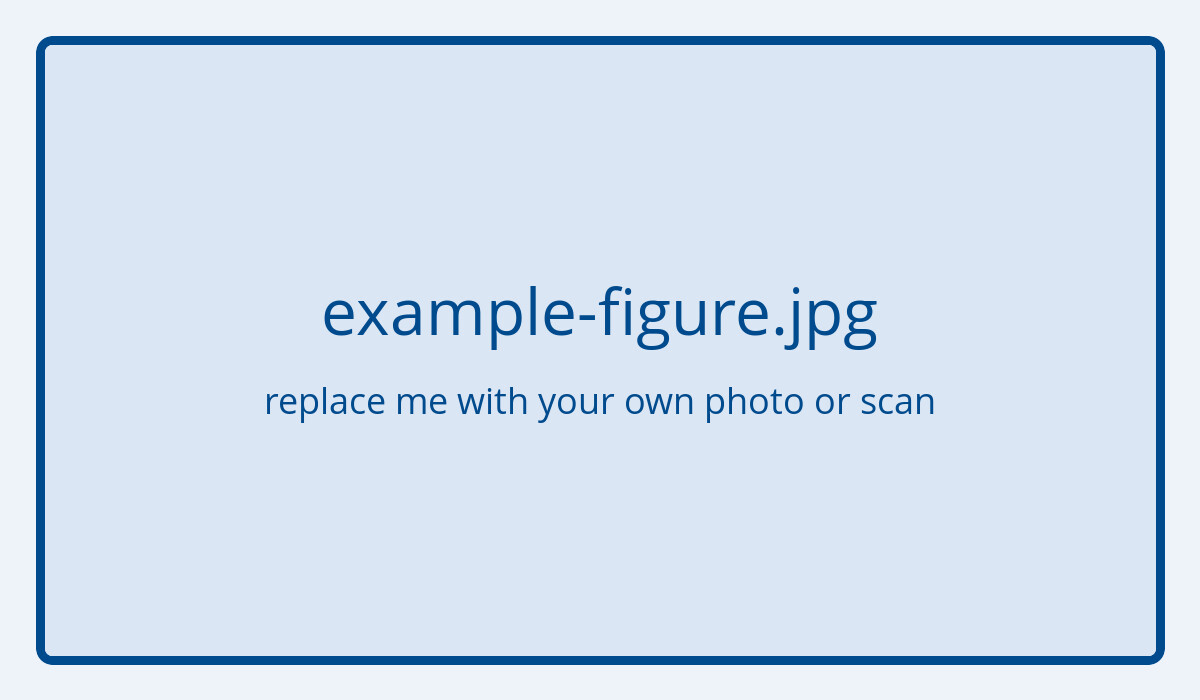
\includegraphics[width=\linewidth]{example-figure.jpg}
  \captionof{figure}{Startup connection dialog: API URL + X-API-Key.}
  \label{fig:fe-connect}
\end{minipage}\hfill
\begin{minipage}[t]{0.47\linewidth}\centering
  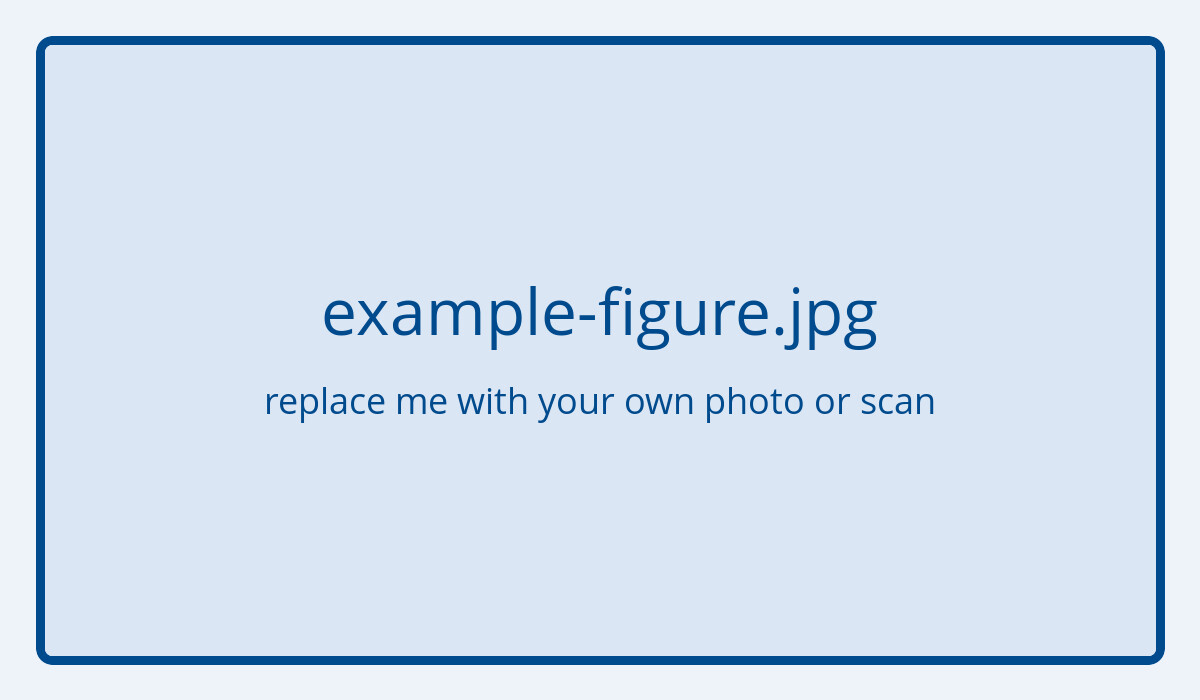
\includegraphics[width=\linewidth]{example-figure.jpg}
  \captionof{figure}{Main screen: <<< list/table, calls \texttt{GET /<<<…>>>} >>>.}
  \label{fig:fe-main}
\end{minipage}

\vspace{1em}

\begin{minipage}[t]{0.47\linewidth}\centering
  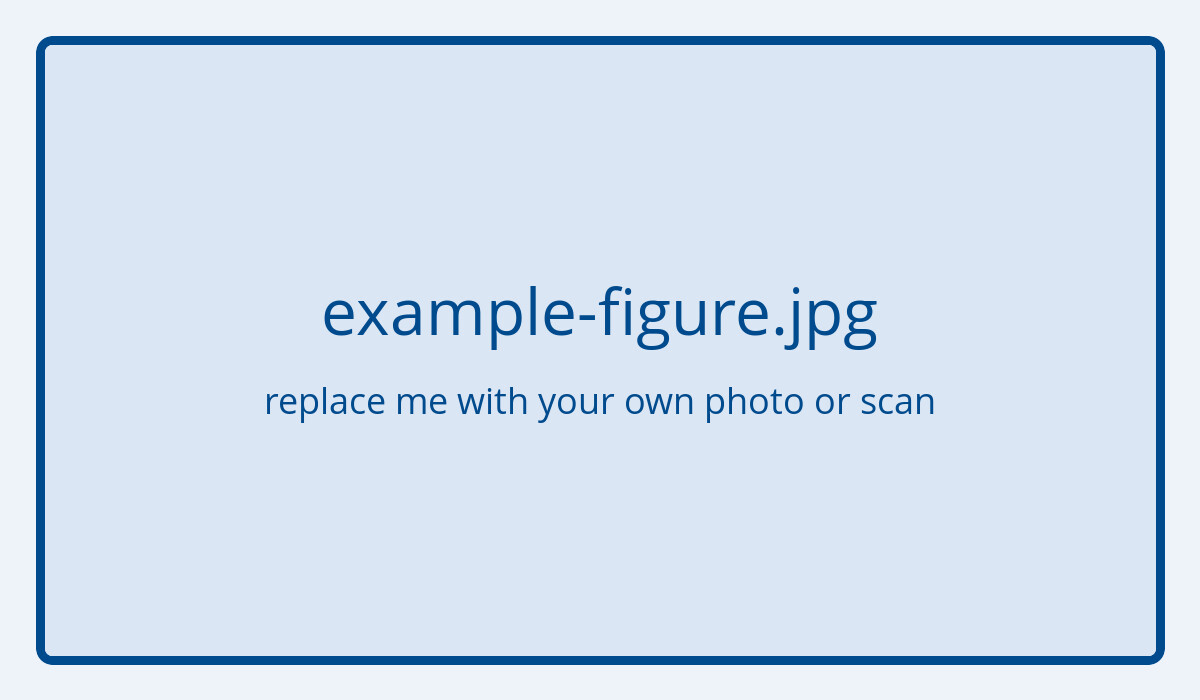
\includegraphics[width=\linewidth]{example-figure.jpg}
  \captionof{figure}{Detail form: <<< create/edit, calls \texttt{POST /<<<…>>>} >>>.}
  \label{fig:fe-detail}
\end{minipage}\hfill
\begin{minipage}[t]{0.47\linewidth}\centering
  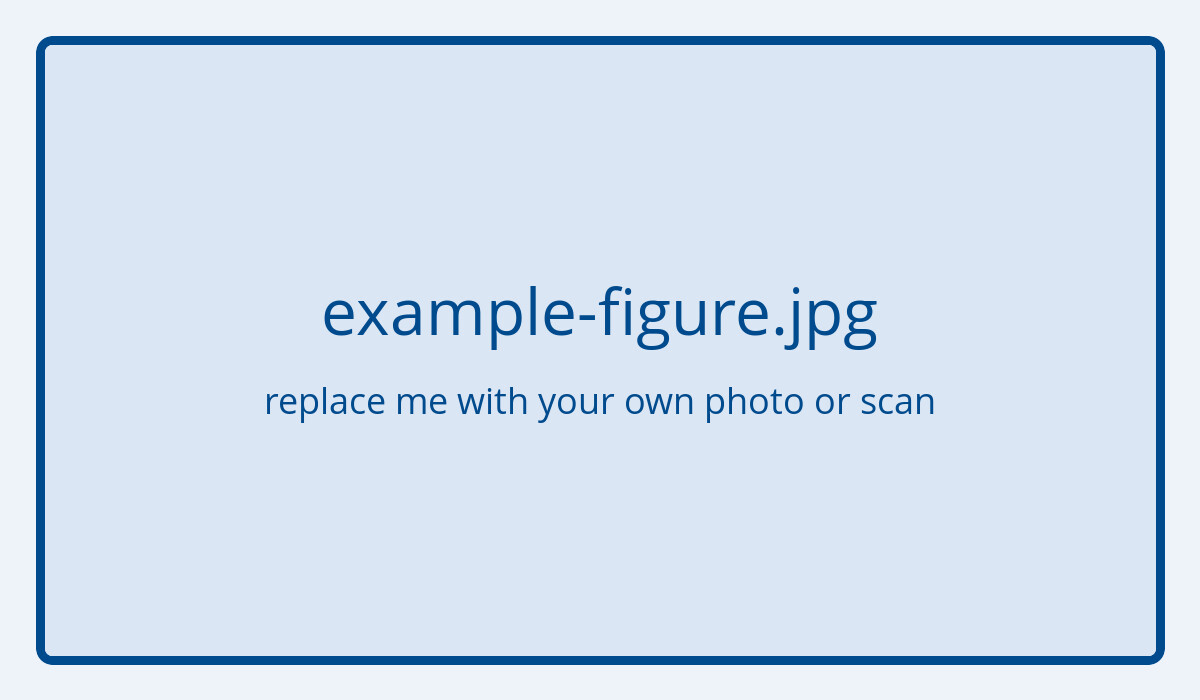
\includegraphics[width=\linewidth]{example-figure.jpg}
  \captionof{figure}{<<< Second feature screen and the endpoint it calls >>>.}
  \label{fig:fe-second}
\end{minipage}
\end{figure}

Figures~\ref{fig:fe-connect}--\ref{fig:fe-second} show the four screens of the
prototype. Figure~\ref{fig:fe-connect} shows <<< the connection dialog that
collects the API URL and X-API-Key at startup >>>; Figure~\ref{fig:fe-main}
shows <<< the main screen and the endpoint it reads from >>>;
Figure~\ref{fig:fe-detail} shows <<< the form used to create/edit a record and
the write endpoint it calls >>>; and Figure~\ref{fig:fe-second} shows <<< the
remaining screen >>>.

% ============================================================
\section{Operation with Docker Compose}
% ============================================================

<<< Which services run in your docker-compose.yml (at least postgres and api)?
Where do the credentials live (.env)? How is the backend deployed on the
lecture server? >>>

% ============================================================
\section{Scope, milestones and risks}
% ============================================================

\textbf{Scope.} <<< How many tables and endpoints? >>>

\textbf{Milestones and schedule.} <<< Fill in the week and the estimated hours;
the hours should add up to roughly 40. >>>

\renewcommand{\arraystretch}{1.2}
\begin{tabularx}{\linewidth}{@{}p{1.4cm}Xp{1.8cm}@{}}
\toprule
\textbf{Week} & \textbf{Milestone} & \textbf{Est. hours} \\
\midrule
<<<1>>>   & <<< e.g. schema + seed data ready >>>                        & <<<8>>> \\
<<<2--3>>> & <<< e.g. API reading/writing, protected by X-API-Key >>>   & <<<12>>> \\
<<<4--5>>> & <<< e.g. frontend operates the core endpoints, .deb >>>    & <<<10>>> \\
<<<6>>>   & <<< e.g. tests + documentation + video >>>                  & <<<10>>> \\
\bottomrule
\end{tabularx}

\textbf{Risks.} <<< One or two risks that could make the project fail. >>>

% ============================================================
\section{Acceptance criteria and testing}
% ============================================================

<<< State when your system counts as ``done and correct'', and how you prove it.
Formulate each criterion as a checkable statement, then name the test that backs
it. Turn the risk above into at least one concrete test case. >>>

\textbf{Acceptance criteria.} <<< Checkable statements about the finished system. >>>
\begin{itemize}[topsep=2pt]
  \item <<< e.g. A record that violates a constraint is rejected (API returns 4xx). >>>
  \item <<< e.g. GET /<<<…>>> returns the correct aggregated value (JOIN + aggregation). >>>
  \item <<< e.g. Write endpoints without a valid X-API-Key are refused (401/403). >>>
\end{itemize}

\textbf{Test plan.} <<< What you test and with which tools. A short list is enough. >>>
\begin{itemize}[topsep=2pt]
  \item \textbf{Database:} <<< which constraints (PK/FK/UNIQUE/NOT NULL) you verify. >>>
  \item \textbf{API:} <<< endpoint tests, happy path + error cases, e.g. with
        \texttt{pytest} and FastAPI's \texttt{TestClient} against a test database (L 08). >>>
  \item \textbf{Business rule:} <<< the test that covers the risk named above. >>>
\end{itemize}

\vspace{1em}
\begin{infobox}
\textbf{Effort budget:} the whole term project (system, documentation and video)
should fit into roughly \textbf{40\,h of work} over at most \textbf{2 months}.
Keep your scope within that budget.
\end{infobox}

\end{document}
